
\section{Supplementary Material}

Randomized Self Organizing Map \\ 
Nicolas P. Rougier$^{1,2,3}$ and Georgios Is. Detorakis$^4$ \\
$^1$ Inria Bordeaux Sud-Ouest \\
$^2$ Institut des Maladies Neurodégénératives, Université  de Bordeaux, CNRS UMR 5293 \\
$^3$ LaBRI, Université de Bordeaux, Institut Polytechnique de Bordeaux, CNRS UMR 5800 \\
$^4$ adNomus Inc., San Jose, CA, USA \\


\noindent\textbf{Abstract.} Self-organizing maps usually rely on a predetermined topology
of the neural space (the map), which is either a rectangular or a hexagonal Cartesian grid.
When the intrinsic dimension of  the input space is much higher than the allowed dimension
of the neural space, then the self-organizing map can be ill-formed. To overcome this problem
in  high dimensional input spaces we propose a variation of the self organizing map algorithm,
where we consider random placement of neurons on a high-dimensional manifold. The positions of
the neural units are drawn from a blue noise  distribution thus various topologies can be
derived. These topologies possess  random (but controllable) discontinuities that allow for a
more flexible self-organization, especially with high-dimensional data. The proposed algorithm
has been tested on one-, two- and \gid{three-dimensions tasks as well as on MNIST handwritten
digits dataset. Furthermore, we investigate the reorganization of the self-organizing maps when
we either remove or add neurons to the map. To analyze the results we use spectral analysis and
Topological Data Analysis tools}. \par

\renewcommand\thefigure{S\arabic{figure}} 
\setcounter{figure}{0} 



\subsection{One dimensional data -- Experiment ${\bf 1}$}



\subsection{Two-dimensional data -- Experiment ${\bf 2}$a}



\begin{figure}[!htpb]
     \centering
     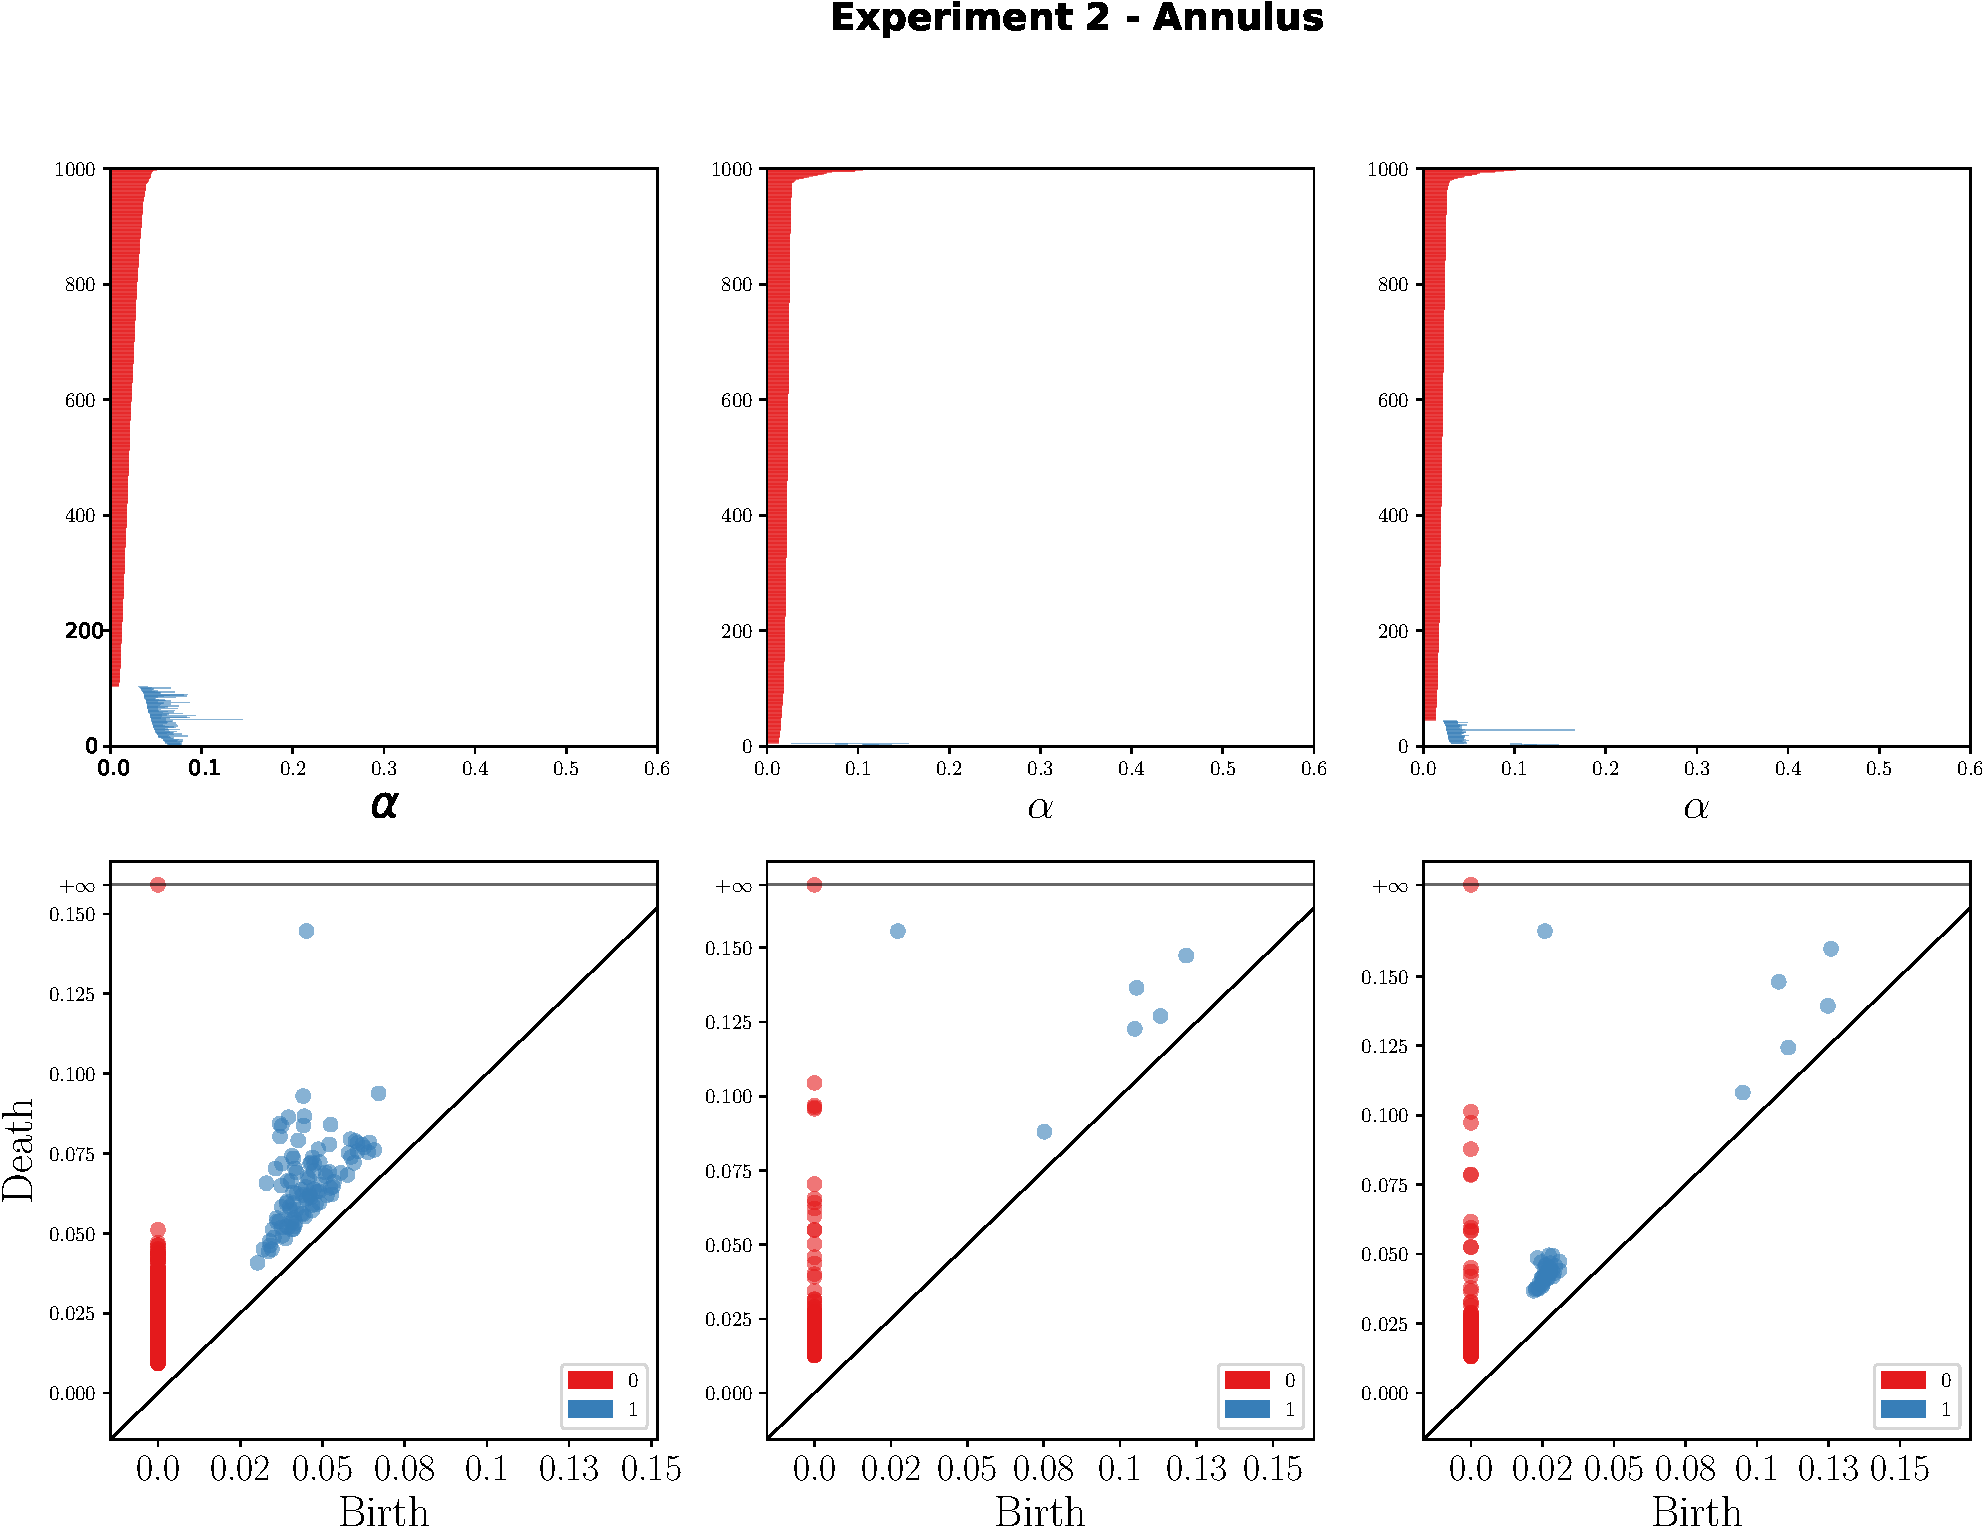
\includegraphics[width=\textwidth]{figures/experiment-2-pd.pdf}
     \caption{{\bfseries \sffamily Persistent Barcode and Diagram for 
     Experiment ${\bf 2}$a.} $2$D uniformly distributed points of an annulus are being used 
     as input to the Kohonen and VSOM learning algorithms. We compute the persistence 
     barcode and diagram of the input samples (first column) top and bottom panels, respectively. 
     The middle column indicates the barcodes and the persistence diagram of the Kohonen
     map the right column the barcodes and the persistence diagram of the VSOM. We observe
     that the topology of the neural space generated by VSOM approaches closer the topology
     of the input space than Kohonen does. The upper row shows the persistence barcodes and
     the bottom row the persistence diagrams. }%
     \label{Fig:persistence_exp2}
\end{figure}

\begin{table}[!ht]
  \begin{center}
    \begin{tabular}{ccccc}
        \textbf{Algorithm} & $d_b$ $H0$ & $W_p$ $(H0)$ & $d_b$ $H1$ & $W_p$ $(H1)$ \\
        \hline
        Kohonen & 0.0522 & 0.0233 & 5.2965 & 2.3564 \\
        VSOM    & 0.0501 & 0.0246 & 4.5197 & 2.3669
      \end{tabular}
      \caption{\textbf{Experiment $2$a Persistence Diagram Distances.} Bottleneck 
      and Wasserstein distances between the persistence diagrams of the input and 
      Kohonen and VSOM. In this experiment both the Kohonen and the VSOM do not express
      any significant difference. $d_b$ is the bottleneck distance~\eqref{eq:bottle},
      $W_p$ is the Wasserstein distance~\eqref{eq:wasser}, $H0$ indicates the Homology Group $0$
      (path-connected components, or one-dimensional holes), $H1$ is the Hologoy group $1$ 
      (two-dimensional holes).}
      \label{table:parameters}
  \end{center}
\end{table}


\subsection{Distributions of Eigenvalues}

\begin{figure}[!htpb]
     \centering
     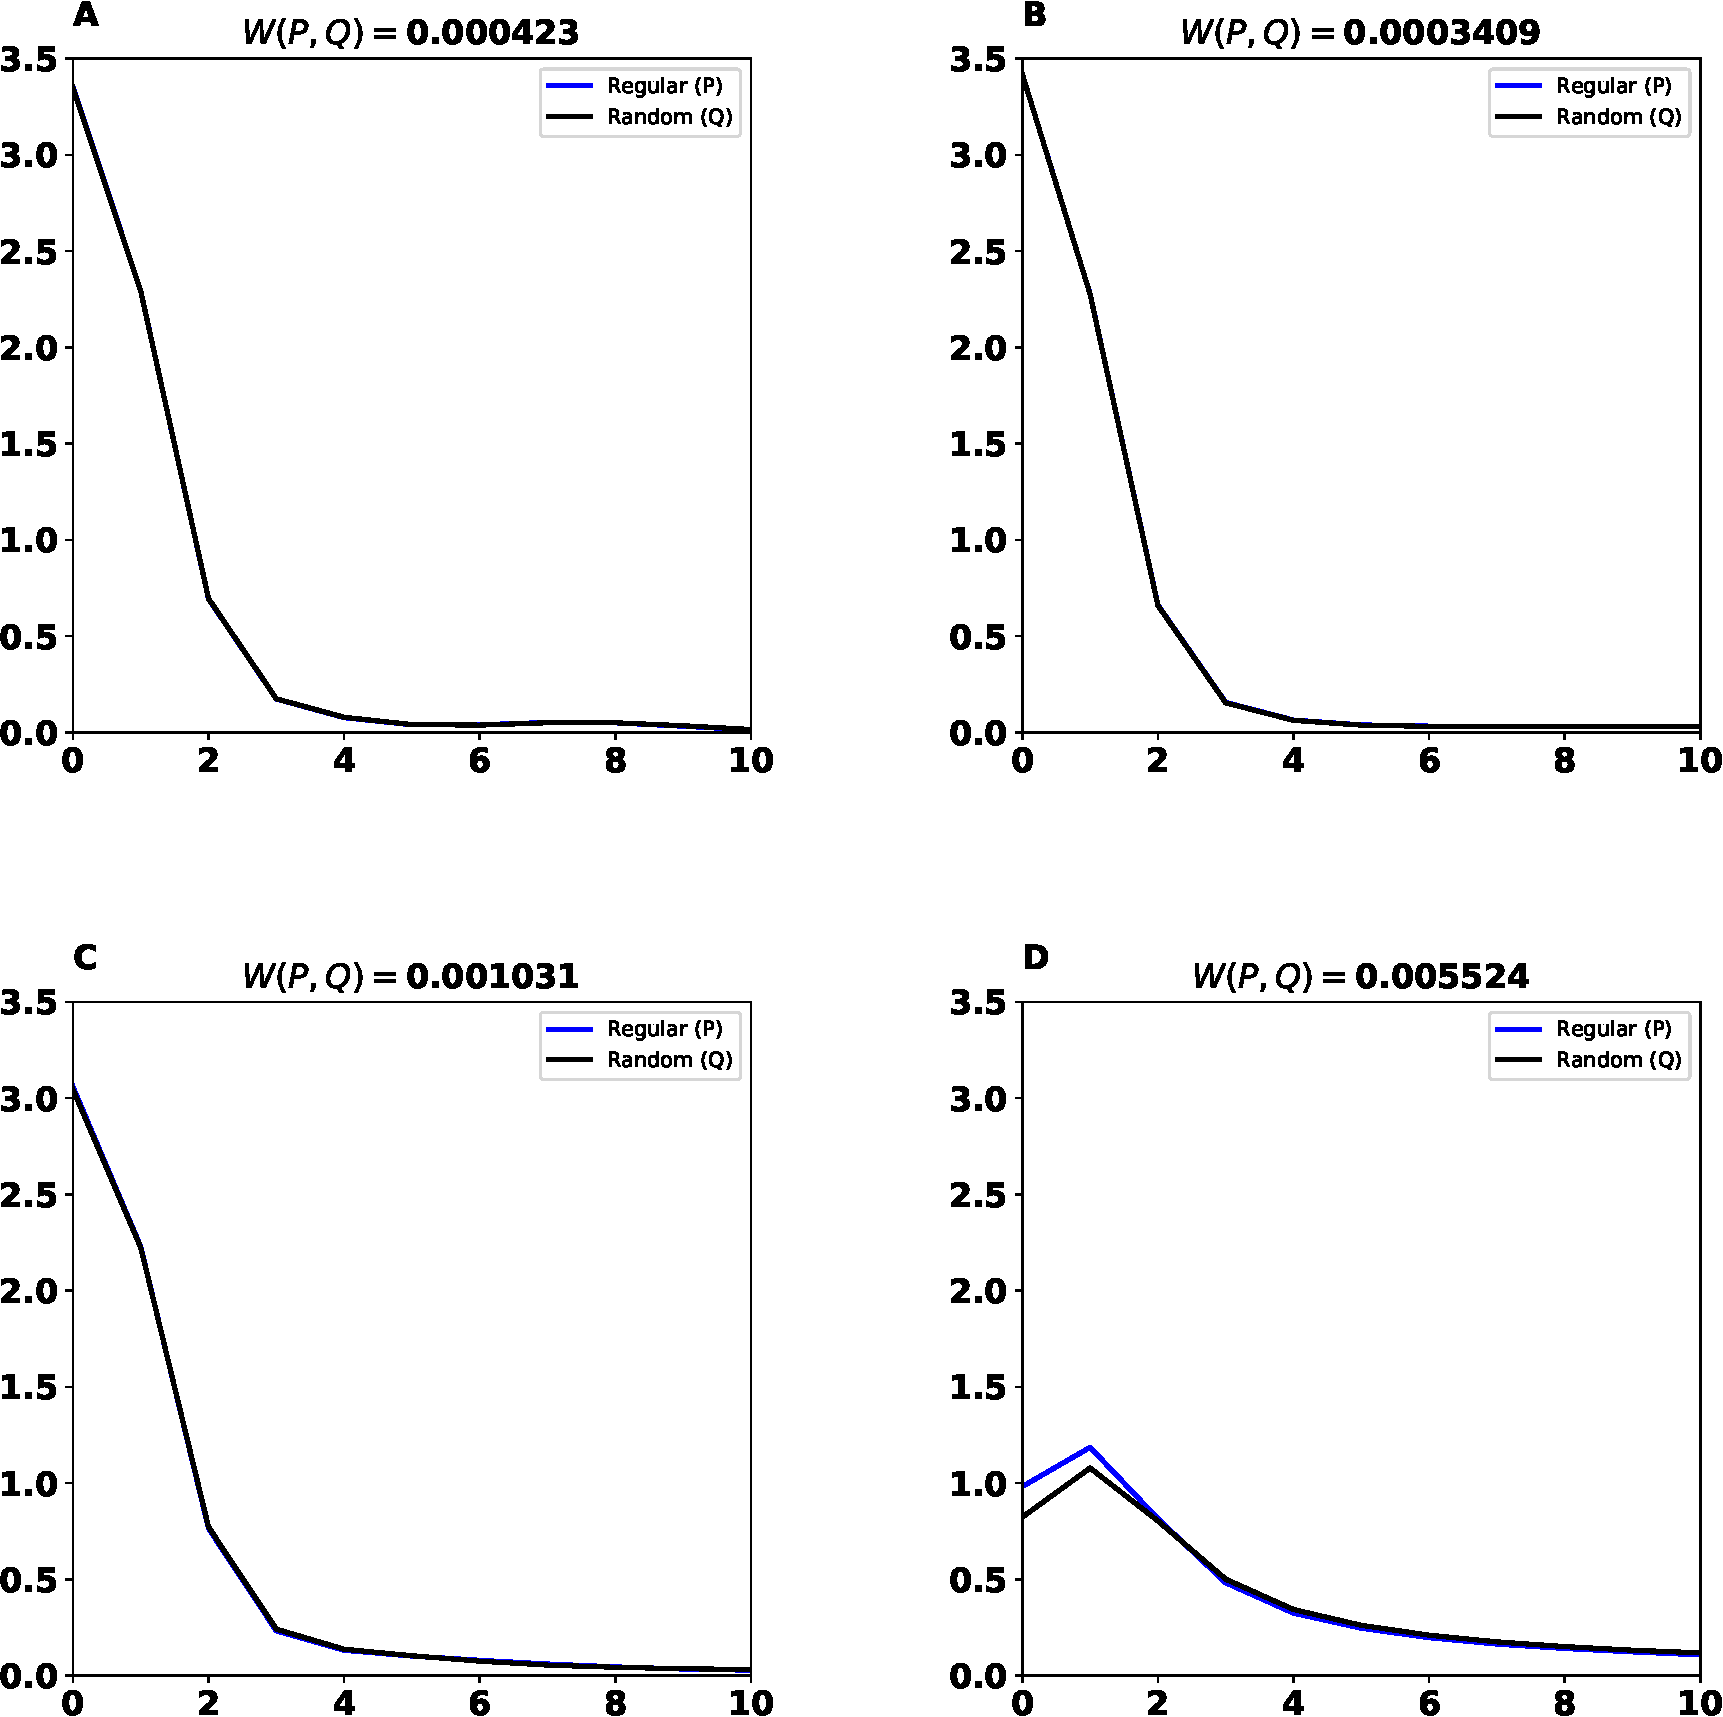
\includegraphics[width=\textwidth]{figures/eig-distributions.pdf}
     \caption{{\bfseries \sffamily Eigenvalues Distributions}
     {\bfseries \sffamily A} Experiment $2$a, a two-dimensional SOM
     maps a two-dimensional uniform annulus distribution\@.
     {\bfseries \sffamily B} Experiment $2$b a two-dimensional uniform
     distribution with holes is the input space for a two-dimensional SOM\@. 
     {\bfseries \sffamily C} Experiment $3$ A two-dimensional SOM learns the
     representations of a three-dimensional uniform distribution (cube).
     {\bfseries \sffamily D} Experiment $4$ A two-dimensional map learns
     the representations of MNIST handwritten data set.
     In all panels blue color indicates the standard Kohonen SOM and the 
     black color shows the VSOM.}%
     \label{Fig:distributions}
\end{figure}


\subsection{Two-dimensional data -- Experiment ${\bf 2}$b}

\begin{figure}[!htpb]
     \centering
     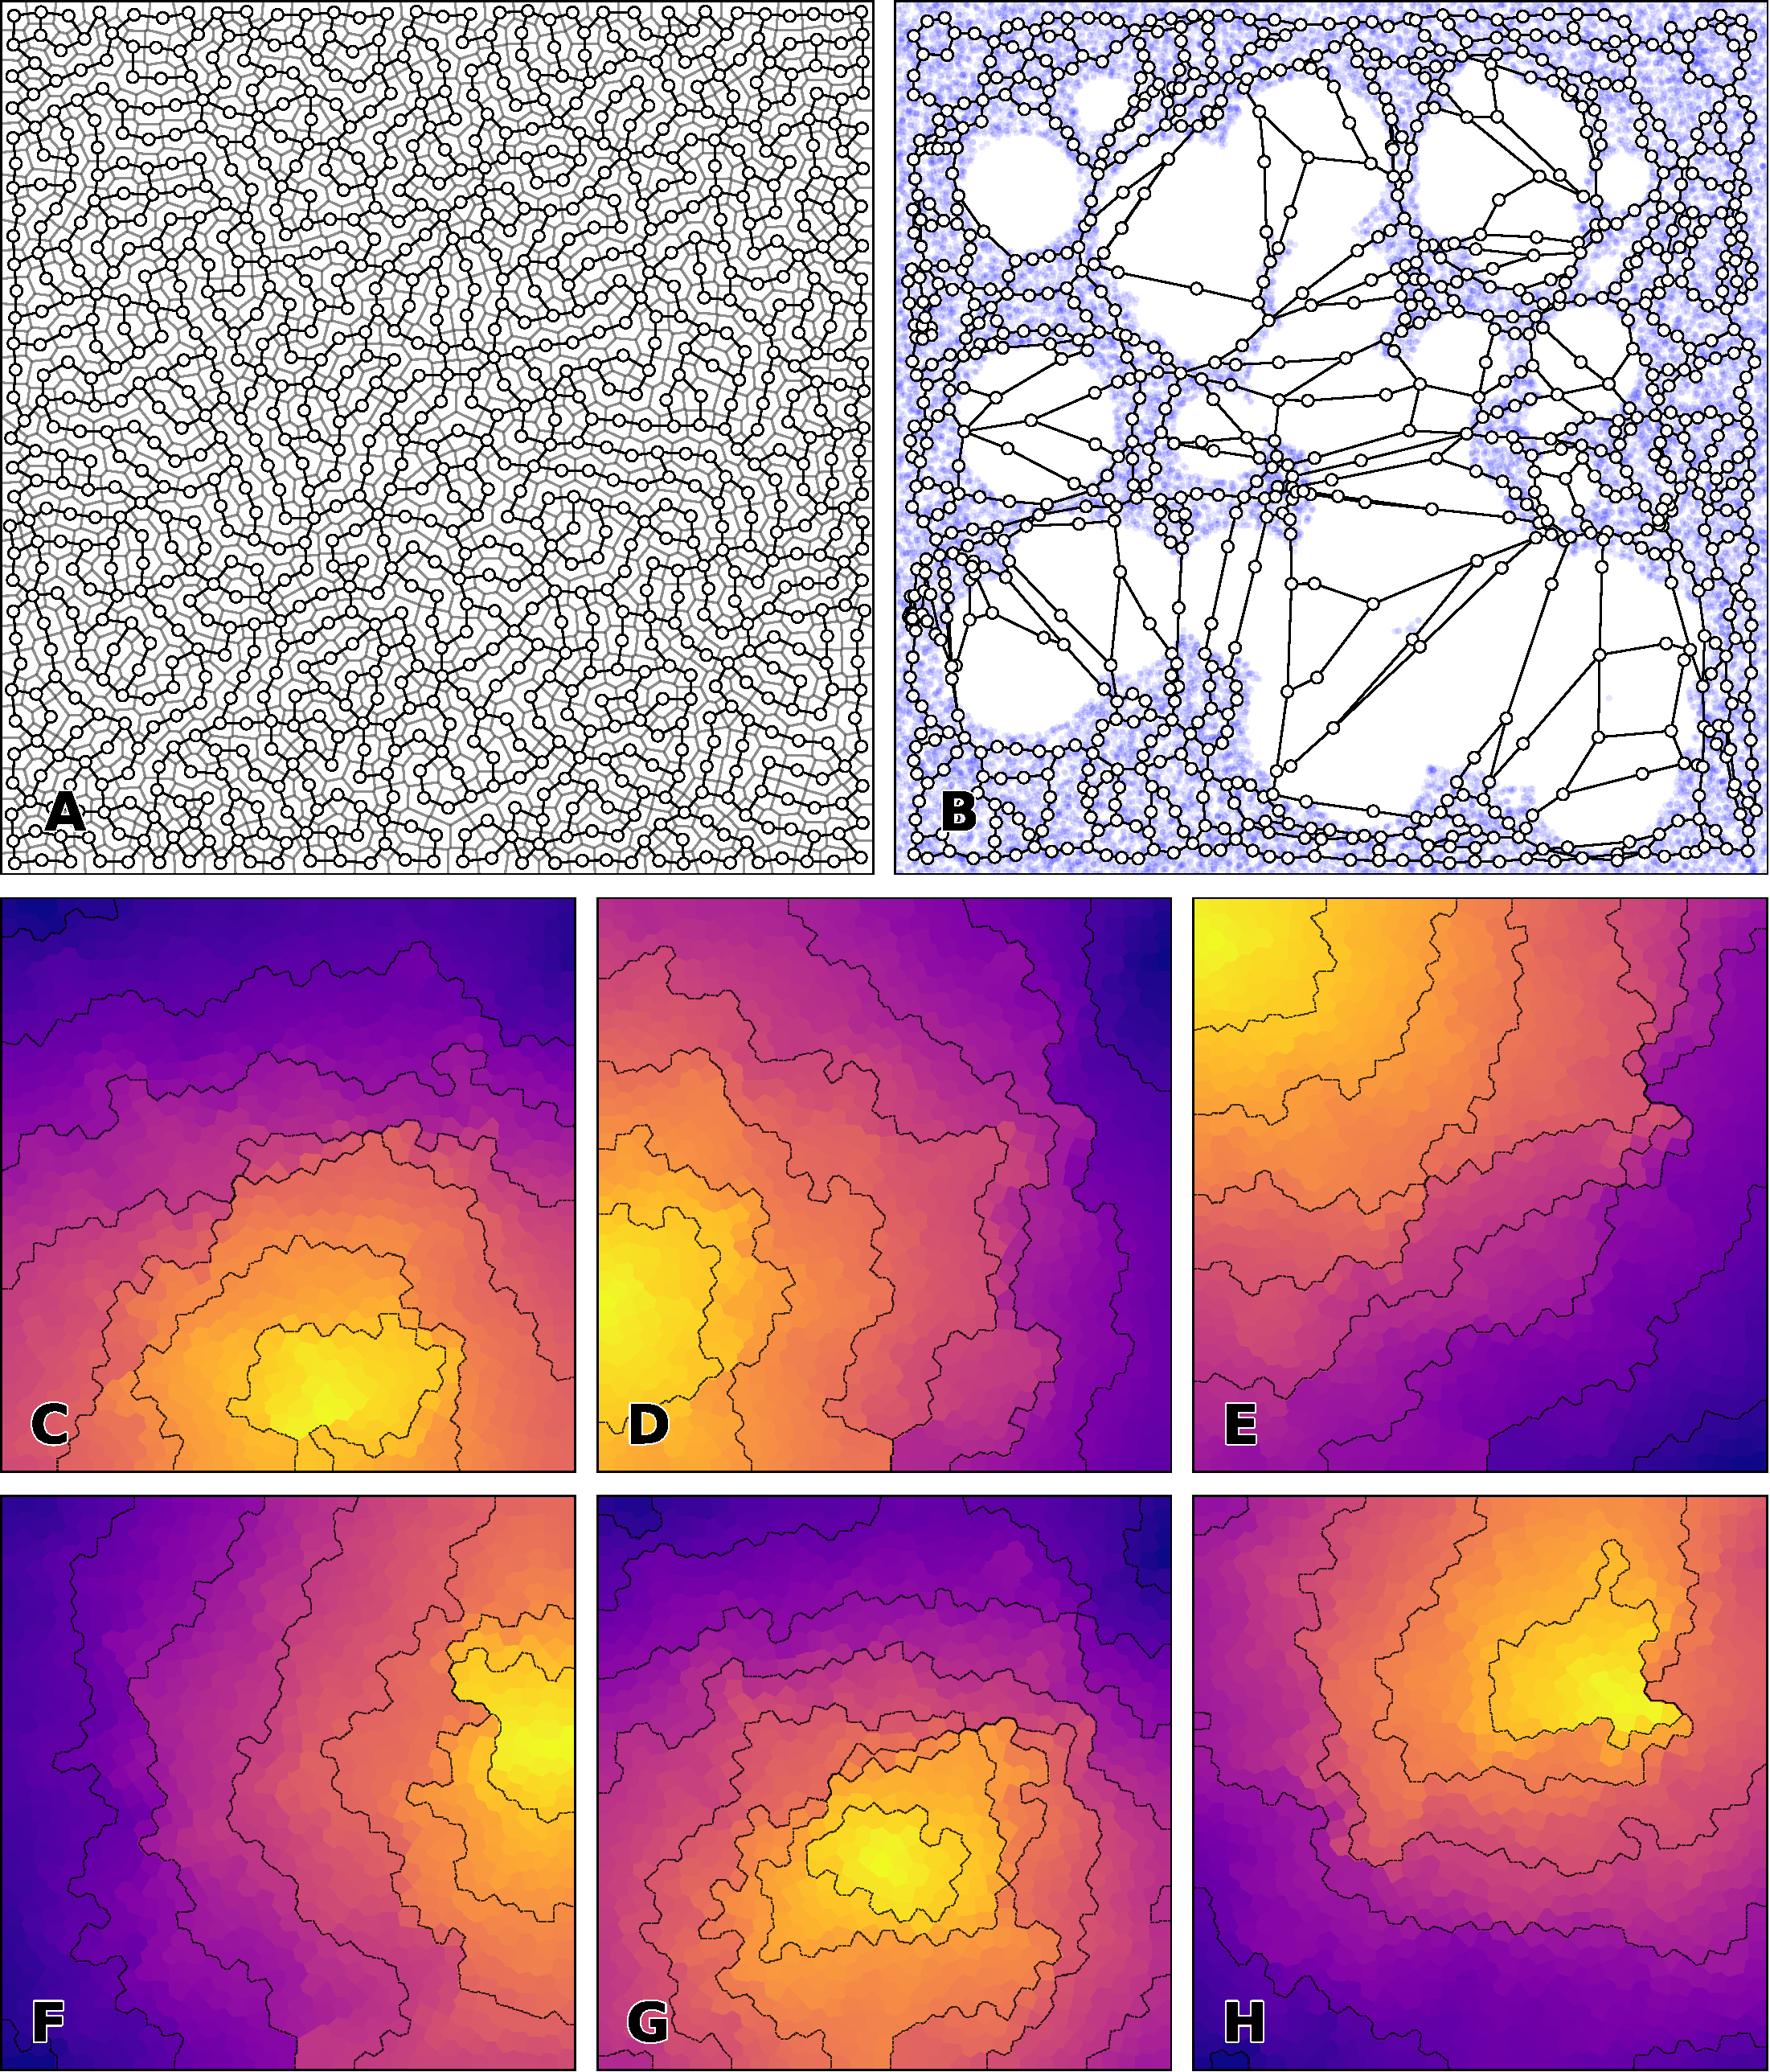
\includegraphics[width=\textwidth]{figures/experiment-2-bis-random-crop.pdf}
     \caption{{\bfseries \sffamily Experiment $2$b -- Uniform distribution on a plane with holes.}
     Voronoidal SOM made of $1024$ neurons with a $2$-nearest neighbors
     induced topology. Model has been trained for $25,000$ epochs on two-dimensional
     points drawn from a uniform distribution on the Cartesian plane $[0, 1] \times [0, 1]$. 
     \textbf{A} Map topology in neural space. \textbf{B} Map prototypes displayed 
     in neural space using Voronoi cells (whose color indicates prototype according 
     to colormap). \textbf{C to H} Map activity for six neurons.}
     \label{Fig:experiment2b}
\end{figure}

\begin{figure}[!htpb]
     \centering
     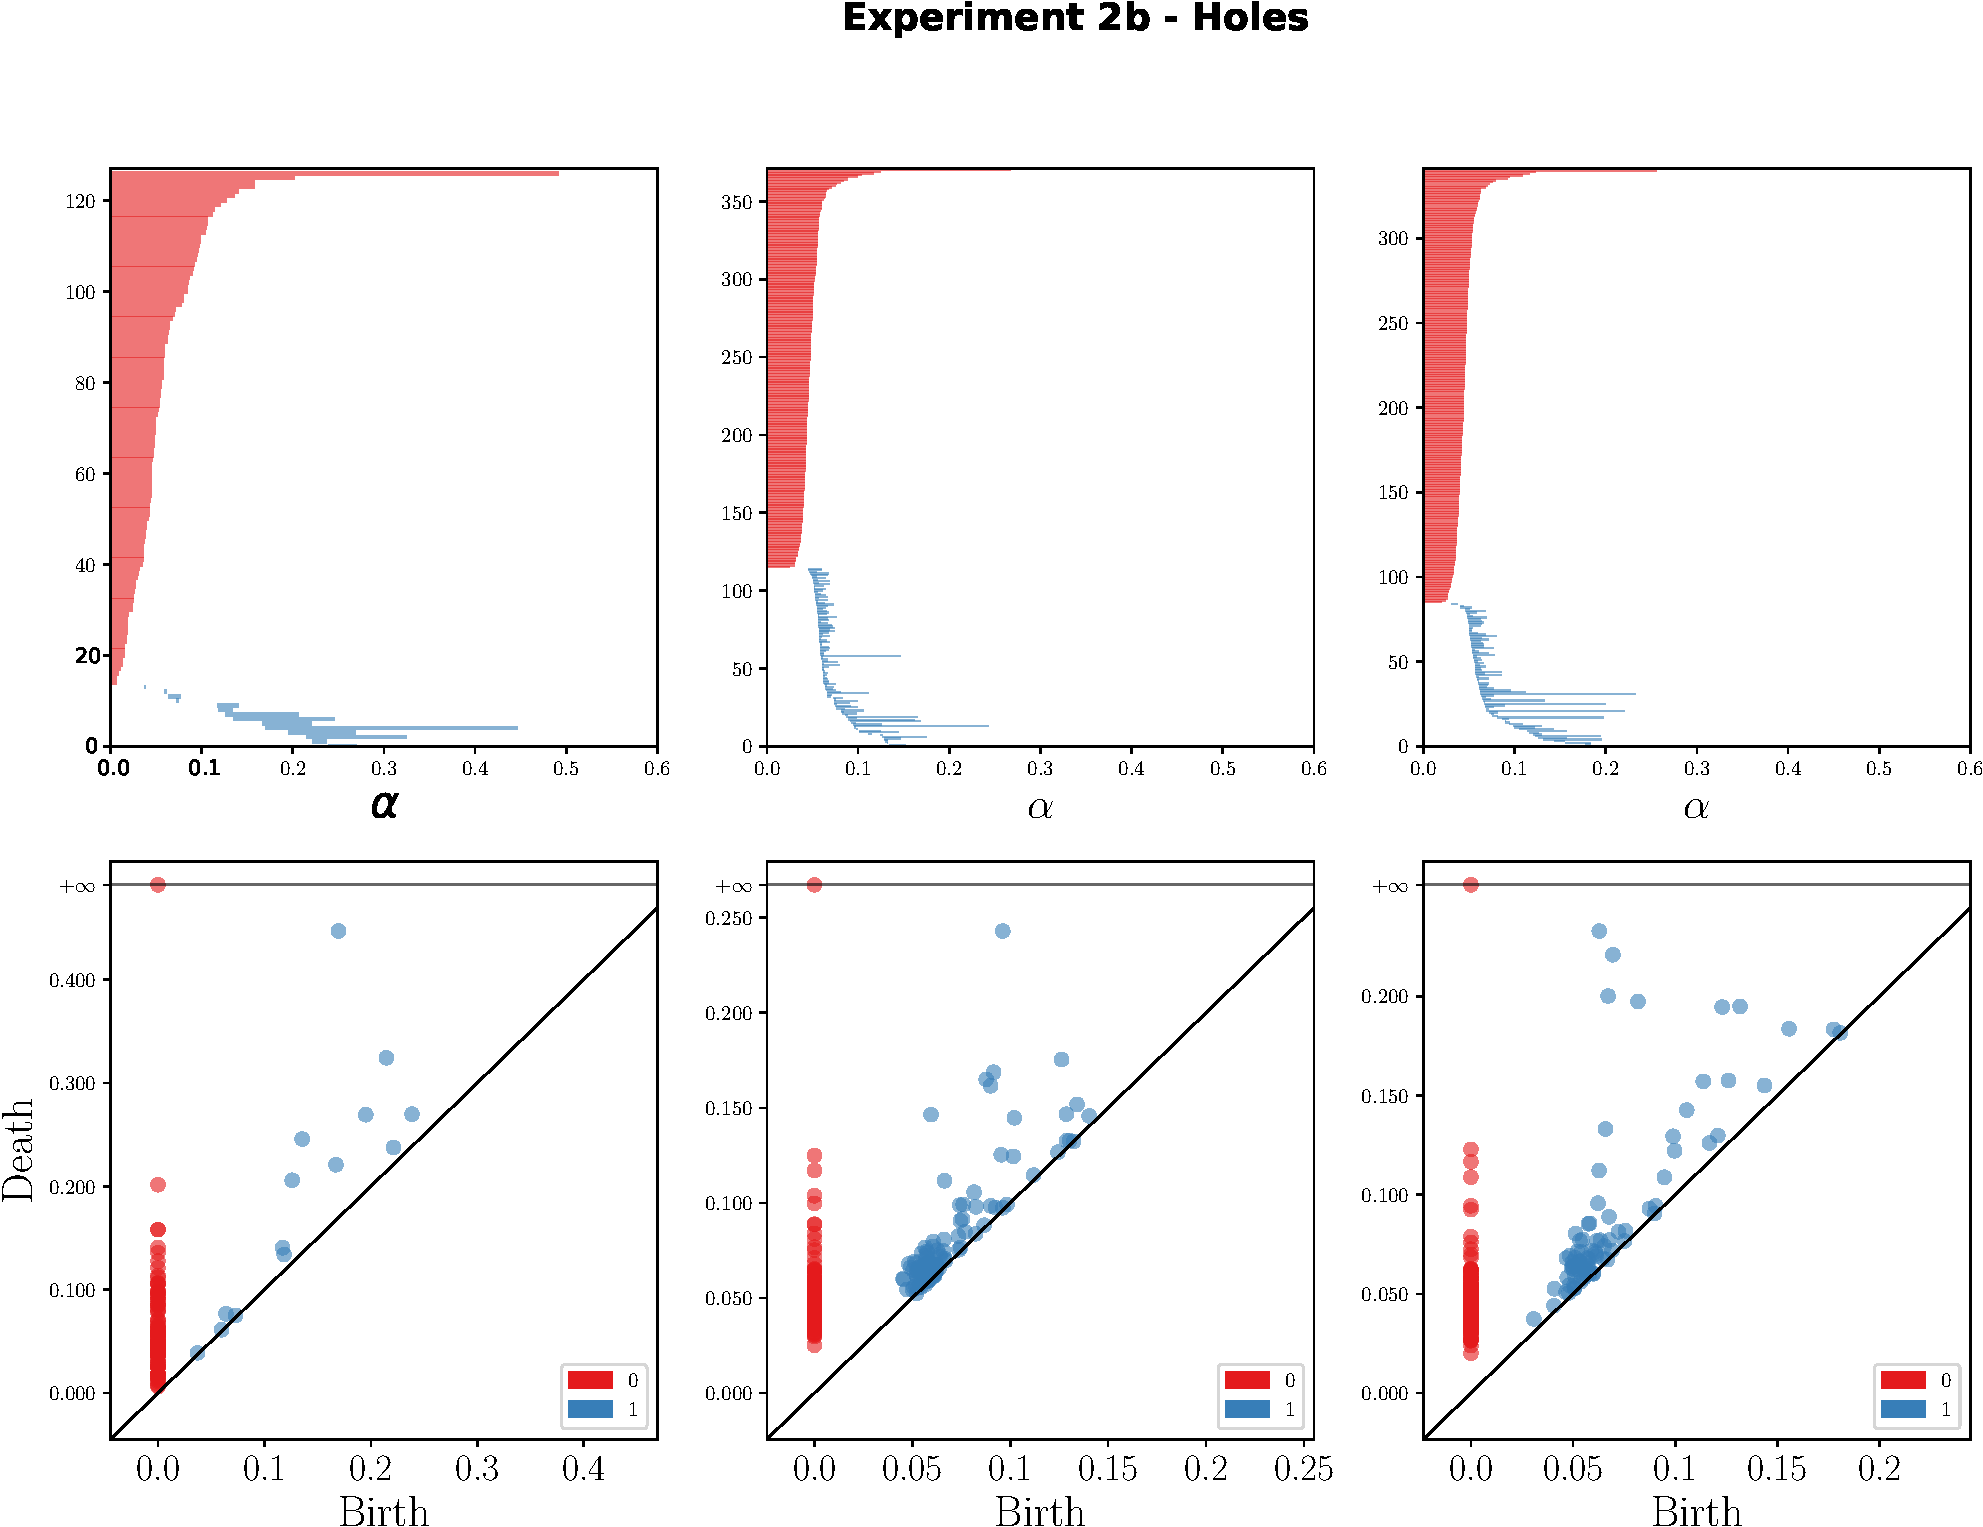
\includegraphics[width=\textwidth]{figures/experiment-2-bis-pd.pdf}
     \caption{{\bfseries \sffamily Persistent Barcode and Diagram for 
     Experiment ${\bf 2}$b.} $2$D uniformly distributed points on a plane with holes 
     are being fed as input to the Kohonen and VSOM learning algorithms. We compute 
     the persistence barcodes and diagrams of the input samples (first column) top and 
     bottom panels, respectively, as well as of the Kohonen map (middle column) and of
     the VSOM (last column). 
     We observe that the topology of the neural space generated by VSOM approaches closer
     the topology of the input space than Kohonen does. The upper row shows the persistence
     barcodes and the bottom row the persistence diagrams. }
     \label{Fig:persistence_exp2b}
\end{figure}

\begin{table}[!ht]
  \begin{center}
    \begin{tabular}{ccccc}
        \textbf{Algorithm} & $d_b$ $H0$ & $W_p$ $(H0)$ & $d_b$ $H1$ & $W_p$ $(H1)$ \\
        \hline
         SOM & 0.0343 & 0.1130 & 6.7631 & 1.5311 \\
        RSOM & 0.0390 & 0.1130 & 5.7588 & 1.4158
      \end{tabular}
      \caption{\textbf{Experiment $2$b Persistence Diagram Distances.} Bottleneck 
      and Wasserstein distances between the persistence diagrams of the input and 
      Kohonen and VSOM. In this experiment both the Kohonen and the VSOM do not express
      any significant difference. $d_b$ is the bottleneck distance~\eqref{eq:bottle},
      $W_p$ is the Wasserstein distance~\eqref{eq:wasser}, $H0$ indicates the Homology Group $0$
      (path-connected components, or one-dimensional holes), $H1$ is the Hologoy group $1$ 
      (two-dimensional holes).}
      \label{table:parameters}
  \end{center}
\end{table}